\documentclass[../../InformazioneQuantistica.tex]{subfiles}

\begin{document}

\section{Misure generalizzate}
\lesson{7 \orangedot}{20/3/2019}
Il formalismo delle \q{evoluzioni generalizzate} ci permette di trattare una classe più ampia di misurazioni.\\
Finora, infatti, abbiamo identificato la misura di uno stato quantistico come una \textit{misura ideale di prima specie}, che corrisponde ad una proiezione di Von Neumann.\index{Misura!di Von Neumann}\\
Matematicamente, consideriamo una funzione d'onda $\ket{\psi(t)}$, e una misura di Von Neumann che a $t=0$ trova che l'osservabile $A$ ha un certo valore $a\in \sigma(A)$. Lo stato del sistema immediatamente dopo la misura è uno stato in cui il valore di $A$ è ben definito, ossia l'autostato di $A$ di autovalore $a$. Per ottenerlo si \textit{proietta} la $\ket{\psi(0)}$ sull'autospazio di $A$ di autovalore $a$:
\begin{align*}
\ket{\psi(0^+)} = \frac{P_a^A \ket{\psi(0)}}{\sqrt{\bra{\psi(0)}P_a^A \ket{\psi(0)}}}
\end{align*}
Perciò una qualsiasi misura \textit{immediatamente successiva} trova per $A$ sempre il valore $a$, con certezza.\\

Potremmo però considerare un \q{processo di misura} con un risultato \textbf{incerto}, per cui lo stato finale è un elemento $\{\ket{\psi_i}\}_{i=1,\dots,N}$ scelto con \textbf{probabilità} $p_i$. Al posto del proiettore usiamo allora una classe più ampia di operatori $\{M_i\}$ \textit{non necessariamente autoaggiunti}, che mappano $\ket{\psi}$ nelle varie possibilità $\ket{\psi_i}$: \marginpar{Misura generalizzata}\index{Misura!Generalizzata}
\begin{align*}
\ket{\psi_i} = \frac{M_i \ket{\psi}}{\sqrt{\bra{\psi_i}M_i^\dag M_i\ket{\psi}}} \qquad p_i = \bra{\psi}M_i^\dag M_i \ket{\psi} \qquad i=1,\dots,N
\end{align*}
Poiché vogliamo che le $\ket{\psi_i}$ esauriscano tutte le possibili evoluzioni di $\ket{\psi}$, si ha che le $p_i$ si sommano a $1$, e quindi: \marginpar{Condizione di completezza}
\begin{align}
\sum_{i=1}^N p_i = 1 \Leftrightarrow \bra{\psi} \sum_{i=1}^N M_i^\dag M_i\ket{\psi} = 1 \Leftrightarrow \bm{\sum_{i=1}^N M_i^\dag M_i = 1}
\label{eqn:condizione-misure}
\end{align}

\textbf{Nota}: se $M_i^\dag = M_i$ ($M_i$ autoaggiunti) e $M_i M_j = \delta_{ij}M_i \Rightarrow M_i^2 = M_i$ ($M_i$ proiettori ortonormali), riotteniamo le \textbf{misure proiettive} (proiezione di Von Neumann), per cui la completezza è data direttamente da $\sum_i M_i = \bb{I}$.

\subsection{Teorema di Neumark}
Si trova che le misure generalizzate sono equivalenti a \textbf{misure proiettive} effettuate in uno \textbf{spazio più grande} dopo una certa \textbf{evoluzione unitaria}.\\

In altre parole, una usuale misura proiettiva su un sistema di $2$ qubit può essere descritta, a livello dei singoli qubit, da una opportuna misura generalizzata.\\

In particolare, il \textbf{teorema di Neumark}\marginpar{Teorema di Neumark}\index{Teorema!Neumark} afferma che l'azione di una misura generalizzata può essere schematizzata come una sequenza di:
\begin{enumerate}
\item \textbf{Ampliamento del sistema}: al sistema $1$ in esame si aggiunge un sistema $2$ ausiliario, detto \textbf{ancilla}\index{Ancilla}, con cui può interagire.
\item \textbf{Evoluzione unitaria} del sistema $1+2$ secondo un qualche operatore $U_{1+2}$
\item \textbf{Misura proiettiva} sul sottosistema $2$ (misura dell'ancilla), osservata dal punto di vista dello stato del sottosistema $1$.
\end{enumerate}

\subsection{Rappresentazione unitaria di Operatori di Kraus}
Avevamo visto che, se consideriamo una matrice densità ridotta $\rho_1$, possiamo vedere ogni sua possibile \textbf{evoluzione generalizzata} come l'applicazione di opportuni \textit{operatori di Kraus}.\\ Nel caso dell'evoluzione temporale, avevamo notato che la rappresentazione di Kraus dell'evoluzione del sottosistema $1$ deriva dall'evoluzione unitaria del sistema composto da $1$ e un sottosistema $2$ (che funge da \textit{ancilla}). Ci chiediamo se ciò sia vero in generale. Possiamo cioè affermare che \textit{ogni} evoluzione generalizzata, descritta da una qualsiasi classe di operatori di Kraus, sia \textit{indotta} dall'evoluzione unitaria di un sistema più grande?

\begin{figure}[H]
    \centering
    \tikzset{every picture/.style={line width=0.75pt}} %set default line width to 0.75pt        
\begin{center}
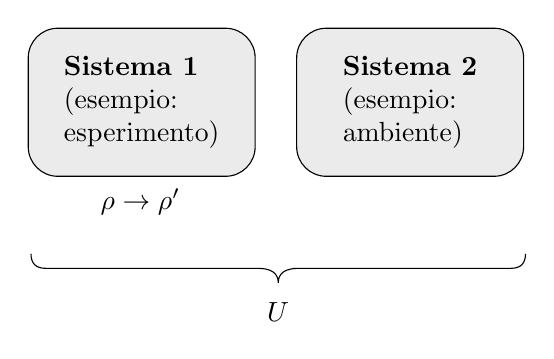
\begin{tikzpicture}[x=0.75pt,y=0.75pt,yscale=-1,xscale=1]
%uncomment if require: \path (0,300); %set diagram left start at 0, and has height of 300

%Rounded Rect [id:dp6009925516212442] 
\draw  [fill={rgb, 255:red, 194; green, 194; blue, 194 }  ,fill opacity=0.33 ] (190.67,114.6) .. controls (190.67,106.72) and (197.05,100.33) .. (204.93,100.33) -- (285.73,100.33) .. controls (293.61,100.33) and (300,106.72) .. (300,114.6) -- (300,157.4) .. controls (300,165.28) and (293.61,171.67) .. (285.73,171.67) -- (204.93,171.67) .. controls (197.05,171.67) and (190.67,165.28) .. (190.67,157.4) -- cycle ;
%Rounded Rect [id:dp13099113646739524] 
\draw  [fill={rgb, 255:red, 194; green, 194; blue, 194 }  ,fill opacity=0.33 ] (320,114.6) .. controls (320,106.72) and (326.39,100.33) .. (334.27,100.33) -- (415.07,100.33) .. controls (422.95,100.33) and (429.33,106.72) .. (429.33,114.6) -- (429.33,157.4) .. controls (429.33,165.28) and (422.95,171.67) .. (415.07,171.67) -- (334.27,171.67) .. controls (326.39,171.67) and (320,165.28) .. (320,157.4) -- cycle ;
%Shape: Brace [id:dp8069175336941659] 
\draw   (192,209) .. controls (192,213.67) and (194.33,216) .. (199,216) -- (301.13,216) .. controls (307.8,216) and (311.13,218.33) .. (311.13,223) .. controls (311.13,218.33) and (314.46,216) .. (321.13,216)(318.13,216) -- (423.25,216) .. controls (427.92,216) and (430.25,213.67) .. (430.25,209) ;

% Text Node
\draw (245.33,136) node  [align=left] {\textbf{Sistema 1}\\(esempio:\\esperimento)};
% Text Node
\draw (374.67,136) node  [align=left] {\textbf{Sistema 2}\\(esempio:\\ambiente)};
% Text Node
\draw (244.67,184.17) node   {$\rho \rightarrow \rho '$};
% Text Node
\draw (311,237) node   {$U$};


\end{tikzpicture}
\end{center}
\end{figure}

Il quesito è per certi versi analogo a quello affrontato nel discutere la \textit{purificazione} di uno stato misto, e procediamo in maniera simile.\\
Partendo dalla mappa $U_1:\rho_1\mapsto \rho_1'$ vogliamo allora trovare l'evoluzione unitaria $U_{1+2}$ che agisce su $\rho_{12}$ inducendo $U_1$ per $\rho_1$. In altre parole, vogliamo interpretare una generica \q{evoluzione generalizzata} $U_1$ come un'evoluzione unitaria $U_{1+2}$ di un sistema più ampio osservata da una delle sue parti.\\

Distinguiamo due casi:
\begin{itemize}
\item Il sottosistema $1$ evolve \textbf{unitariamente} tramite $U_1$. Ma allora una $U_{1+2}: \hs_1 \otimes \hs_2 \to \hs_1 \otimes \hs_2$ unitaria che agisce sul sistema $1+2$ è  data da:
\begin{align*}
U_{1+2} = U_1 \otimes \bb{I}_2
\end{align*}
\textbf{Dimostrazione}.
Supponiamo che lo stato iniziale di $1$ sia $\ket{\psi}_1$ puro, e quello di $2$ sia $\ket{0}_2$. $U_{1+2}$ è il prodotto tensore tra una matrice unitaria e l'identità, e quindi è unitario. Si verifica immediatamente che tale $U_{1+2}$ induce l'evoluzione data da $U_1$ per $\rho_1$:
\begin{align*}
\rho_1' &= \underset{2}{\op{Tr}}(\rho_{12}(t)) = \underset{2}{\op{Tr}}(U_{1+2}\ket{\psi}_1\ket{0}_{2}\bra{\psi}_1\bra{0}_{2}U_{1+2}^\dag)=\\
&= \sum_{k=1}^{\op{dim}\hs_2} \bra{k}_2 \left(U_1 \otimes \bb{I}_2\right)\ket{\psi}_1\ket{0}_{2}\bra{\psi}_1\bra{0}_{2}\left(U_1^\dag \otimes \bb{I}_2\right)\ket{k}_2 =\\
&=\sum_{k=1}^{\op{dim}\hs_2} \braket{k|0}\braket{0|k} U_1 \ket{\psi}_1 \bra{\psi}_1 U_1^\dag =U_1 \rho_1 U_1^\dag
\end{align*}
Il risultato si generalizza anche considerando per $\rho_1$ un generico stato misto, dato che vale $\rho_1 = \sum_n p_n\ket{\phi_n}\bra{\phi_n}$ e le operazioni svolte nella dimostrazione (evoluzione unitaria e traccia) sono tutte lineari. Analogamente, non è richiesto che $\rho_2$ corrisponda ad uno stato puro: se così non è basta estendere $\hs_2$ e purificare lo stato.
\item Il sottosistema $1$ evolve \textbf{non unitariamente}, tramite un processo che può essere rappresentato da operatori di Kraus $\{E_k\}_{k=1,\dots,M}$, $E_k:\hs_1 \to \hs_1$:
\begin{align}
\rho_1' = \sum_{k=1}^M E_k \rho_1 E_k^\dag \qquad \sum_{k=1}^M E_k^\dag E_k = \bb{I}
\label{eqn:def-kraus}
\end{align}
Questo è il caso generale in cui i sottosistemi $1$ e $2$ \textit{interagiscono} durante l'evoluzione. Si trova allora che $U_{1+2}$ in questo caso è dato da:
\begin{align}
U_{1+2}\ket{\psi}_1 \ket{0}_2 = \sum_{k=1}^M (E_k \otimes \bb{I}_2) \ket{\psi}_1 \ket{k}_2
\label{eqn:U-def}
\end{align}
dove $\{\ket{k}_2\}_{k=1}^M$ è una qualsiasi base ON di $\hs_{2}$, con $M=\op{dim}\hs_2$.
\end{itemize}

\textbf{Dimostrazione}. Supponiamo che lo stato iniziale del sistema sia $\ket{\psi}_1\ket{0}_2 \equiv \ket{\psi 0}_{12}$.



Dimostriamo che:
\begin{enumerate}
\item $U_{1+2}$ è unitario. Possiamo vederlo mostrando che preserva le norme:
\begin{align*}
\bra{\psi 0}_{12}U^\dag_{1+2} U_{1+2} \ket{\psi 0}_{12} &\underset{(\ref{eqn:U-def})}{=} \left(\sum_{k=1}^M E_k^\dag \bra{\psi}_1 \bra{k}_2\right)
\left( \sum_{l=1}^M E_l \ket{\psi}_1 \ket{l}_2 \right) =\\
&\underset{(a)}{=} \sum_{k=1}^M \sum_{l=1}^M \underbrace{\braket{k|l}}_{\delta_{kl}} \bra{\psi}_1E_k^\dag E_l \ket{\psi}_1 = \sum_{k} \bra{\psi}E_k^\dag E_k \ket{\psi}=\\
&=\bra{\psi}\sum_k E_k^\dag E_k \ket{\psi} \underset{(\ref{eqn:def-kraus})}{=}\braket{\psi|\psi}=1
\end{align*}
dove in (a) usiamo il fatto che gli $E_k$ agiscono solo su $\hs_1$, ossia sul primo sottosistema, e lasciano invariato il secondo. Tutto ciò vale anche se al posto di $\ket{\psi}$ consideriamo uno stato misto.
\item L'evoluzione dello stato $\rho_{12}$ del sistema composto secondo $U$ \textit{induce} l'evoluzione di $\rho_1$ data dagli operatori di Kraus $\{E_k\}$. Partiamo dal caso in cui $\rho_1$ descrive uno stato puro, ossia $\rho_1 = \ket{\psi}\bra{\psi}$. Allora si ha:
\begin{align*}
\rho_1' &= \underset{2}{\op{Tr}}\left(\rho_{12}(t)\right)=\underset{2}{\op{Tr}}(U_{1+2}\ket{\psi 0}_{12}\bra{\psi0}_{12}U^\dag_{1+2}) = \\
&= \sum_{k=1}^M \bra{k}_2\left(\sum_{l=1}^M E_l \ket{\psi}_1\ket{l}_2\right) \left(\sum_{m=1}^M \bra{\psi}_1 \bra{m}_2 E_m^\dag\right)\ket{k}_2 =\\
&= \sum_{k,l,m=1}^M  \underbrace{\braket{k|l}}_{\delta_{kl}}\underbrace{\braket{m|k}}_{\delta_{km}}
E_l \ket{\psi}_1 \bra{\psi}_1 E_m^\dag = \sum_{k=1}^M E_k \ket{\psi}_1\bra{\psi}_1E_k^\dag =
\\
&= \sum_{k=1}^M E_k \rho_1 E_k^\dag
\end{align*}
Nel caso invece $\rho_1$ descrivesse uno stato misto, tale risultato continua a valere: avremo infatti $\rho_1 = \sum_i p_i \ket{\psi_i}\bra{\psi_i}$, e sfruttando la \textbf{linearità} dei passaggi svolti nella dimostrazione, si arriva sempre alla tesi del teorema.
\end{enumerate}

\subsection{Motivazione delle misure generalizzate}
Abbiamo visto come un'evoluzione unitaria su un sistema grande si traduce in un'evoluzione generalizzata sui sottosistemi di cui è composto (e viceversa).\\
Analogamente, si trova che una \textbf{misura proiettiva} sul sistema composto si traduce in una \textbf{misura generalizzata} sui suoi sottosistemi. In generale, perciò, misure proiettive su un sistema non sono più proiettive se esaminate dal punto di vista delle singole parti.\\


\begin{figure}[H]
    \centering
    \tikzset{every picture/.style={line width=0.75pt}} %set default line width to 0.75pt        
\begin{center}
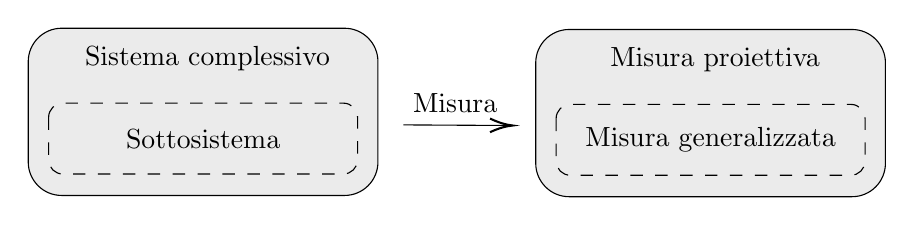
\begin{tikzpicture}[x=0.75pt,y=0.75pt,yscale=-1,xscale=1]
%uncomment if require: \path (0,300); %set diagram left start at 0, and has height of 300

%Rounded Rect [id:dp6106726008236387] 
\draw  [color={rgb, 255:red, 0; green, 0; blue, 0 }  ,draw opacity=1 ][fill={rgb, 255:red, 194; green, 194; blue, 194 }  ,fill opacity=0.33 ] (359.01,102.71) .. controls (359.01,93.81) and (366.22,86.6) .. (375.12,86.6) -- (511.39,86.6) .. controls (520.29,86.6) and (527.5,93.81) .. (527.5,102.71) -- (527.5,151.05) .. controls (527.5,159.95) and (520.29,167.17) .. (511.39,167.17) -- (375.12,167.17) .. controls (366.22,167.17) and (359.01,159.95) .. (359.01,151.05) -- cycle ;
%Rounded Rect [id:dp8954205367068233] 
\draw  [dash pattern={on 4.5pt off 4.5pt}] (368.83,129.52) .. controls (368.83,125.75) and (371.89,122.69) .. (375.66,122.69) -- (510.85,122.69) .. controls (514.62,122.69) and (517.68,125.75) .. (517.68,129.52) -- (517.68,150) .. controls (517.68,153.78) and (514.62,156.83) .. (510.85,156.83) -- (375.66,156.83) .. controls (371.89,156.83) and (368.83,153.78) .. (368.83,150) -- cycle ;
%Rounded Rect [id:dp5246313063373345] 
\draw  [color={rgb, 255:red, 0; green, 0; blue, 0 }  ,draw opacity=1 ][fill={rgb, 255:red, 194; green, 194; blue, 194 }  ,fill opacity=0.33 ] (114.5,102.11) .. controls (114.5,93.21) and (121.71,86) .. (130.61,86) -- (266.88,86) .. controls (275.78,86) and (282.99,93.21) .. (282.99,102.11) -- (282.99,150.45) .. controls (282.99,159.35) and (275.78,166.57) .. (266.88,166.57) -- (130.61,166.57) .. controls (121.71,166.57) and (114.5,159.35) .. (114.5,150.45) -- cycle ;
%Rounded Rect [id:dp909540949537371] 
\draw  [dash pattern={on 4.5pt off 4.5pt}] (124.32,128.92) .. controls (124.32,125.15) and (127.38,122.09) .. (131.15,122.09) -- (266.34,122.09) .. controls (270.11,122.09) and (273.17,125.15) .. (273.17,128.92) -- (273.17,149.41) .. controls (273.17,153.18) and (270.11,156.23) .. (266.34,156.23) -- (131.15,156.23) .. controls (127.38,156.23) and (124.32,153.18) .. (124.32,149.41) -- cycle ;
%Straight Lines [id:da4759430012113268] 
\draw    (295.23,132.57) -- (345.94,132.86) ;
\draw [shift={(347.94,132.87)}, rotate = 180.33] [color={rgb, 255:red, 0; green, 0; blue, 0 }  ][line width=0.75]    (10.93,-3.29) .. controls (6.95,-1.4) and (3.31,-0.3) .. (0,0) .. controls (3.31,0.3) and (6.95,1.4) .. (10.93,3.29)   ;


% Text Node
\draw (445.4,101.27) node  [align=left] {Misura proiettiva};
% Text Node
\draw (443.25,139.76) node  [align=left] {Misura generalizzata};
% Text Node
\draw (200.89,100.68) node  [align=left] {Sistema complessivo};
% Text Node
\draw (198.75,139.16) node  [align=left] {Sottosistema};
% Text Node
\draw (320.18,122.09) node  [align=left] {Misura};


\end{tikzpicture}
\end{center}
\end{figure}

Consideriamo nello specifico un sistema $1+2$ (sistema in esame + ancilla) che viene fatto evolvere unitariamente da $U_{12}$, che come abbiamo visto in (\ref{eqn:U-def}) è legata all'evoluzione generalizzata definita dagli operatori di Kraus $\{E_k\}$ su $1$. Per un sistema che parte da $\ket{\Psi(0)}_{12}=\ket{\psi}_1\ket{0}_2$ otteniamo:
\begin{align*}
\ket{\Psi(t)}_{12}=U_{12}\ket{\psi}_1 \ket{0}_2 = \sum_{k=0}^M E_k \ket{\psi}_1 \ket{k}_2 \Rightarrow \rho_{12}(0)=\ket{\Psi(t)}_{12}\bra{\Psi(t)}_{12}
\end{align*}
Consideriamo una \textbf{misura proiettiva} sul secondo sottosistema per verificare se si trovi o meno nello stato $\ket{i}_2$, e che quindi equivale ad un operatore che proietta la funzione d'onda nel sottospazio generato da $\ket{i}_2$:
\begin{align*}
\hat{P}_i = \bb{I}_1 \otimes \ket{i}_2\bra{i}_2
\end{align*}
Calcoliamo la probabilità di ottenere $i$ dalla misura: %Pag. 287
\begin{align*}
p_i &= \op{Tr}(\rho_{12}(t)\hat{P}_i) = \op{Tr}\left( \left[\sum_{k,k'}^ME_k\ket{\psi}_1\ket{k}_2\bra{\psi}_1\bra{k'}_2E_{k'}^\dag \right](\bb{I}_1 \otimes \ket{i}_2\bra{i}_2)\right) =\\
&= \op{Tr}\left( \sum_{k,k'}^M E_k \ket{\psi}_1 \bra{\psi}_1 E_k^\dag \otimes {\braket{k'|i}}\ket{k}_2 \bra{i}_2\right) =\\
&=\sum_{m=1}^{\op{dim}\hs_1} \sum_{n=1}^{\op{dim}\hs_2} \bra{m}_1 \bra{n}_2 \op{Tr}\left( \sum_{k,k'}^M E_k \ket{\psi}_1 \bra{\psi}_1 E_k^\dag \otimes {\braket{k'|i}}\ket{k}_2 \bra{i}_2\right) \ket{m}_1 \ket{n}_2 = \\
&= \sum_{m,n}^{\op{dim}\hs_{1,2}} \sum_{k,k'}^M \bra{m}_1 E_k \ket{\psi}_1 \bra{\psi}_1 E_k^\dag \ket{m}_1 \underbrace{\braket{n|k}}_{\delta_{nk}}\underbrace{\braket{k'|i}}_{\delta_{k'i}}\underbrace{\braket{i|n}}_{\delta_{in}} = \\
&\underset{(a)}{=} \sum_{m}^{\op{dim}\hs_1} \bra{m}_1 E_i \ket{\psi}_1 \bra{\psi}_1 E_i^\dag \ket{m}_1 \underset{(*)}{=} \sum_{m}^{\op{dim}\hs_1} \bra{\psi}_1 E_k^\dag \underbrace{\ket{m}_1 \bra{m}_1}_{\bb{I}_1} E_i \ket{\psi}_1 = \bra{\psi}_1 E_i^\dag E_i \ket{\psi}_1
\end{align*}
dove in (a) usiamo le $\delta$ di Kronecker per identificare $k'=k=n=i$, \q{collassando} tre sommatorie in un colpo solo.

Al passaggio segnato (*) possiamo anche riscrivere come:
\begin{align*}
p_i = \op{Tr}(E_i \rho_1 E_i^\dag) \underset{(b)}{=} \op{Tr}(\rho_1 E_i^\dag E_i) \equiv \op{Tr}(\rho_1 M_i^\dag M_i)      
\end{align*}
dove in (b) usiamo la ciclicità della traccia, e nel passaggio finale riconosciamo in $E_i$, che generalmente non sono proiettori, gli operatori $M_i$ che avevamo introdotto nel definire le misure generalizzate.\\

\textbf{Riepilogando}, una \textit{evoluzione generalizzata} $S: \rho_1 \to \rho_1'$ di un certo sistema $1$ è sempre indotta dall'evoluzione unitaria su un sistema più grande (e viceversa), dato dall'unione di $1$ con un sottosistema $2$, detto \textit{ancilla}, con cui $1$ può interagire. Possiamo ora effettuare una misura proiettiva su $1$, utilizzando il formalismo di Von Neumann, o una misura proiettiva su $2$, che induce una \textit{misura generalizzata} su $1$ per effetto delle correlazioni tra i due sistemi prodotte (generalmente) dall'evoluzione unitaria. Ciò apre un'intera classe di possibilità in più per esaminare lo stato di $1$, che esamineremo nelle prossime due sezioni.

\subsection{Weak Measurement}
Sfruttando le correlazioni tra i sottosistemi $1$ e $2$ è possibile \textit{estrarre informazioni} da $1$ effettuando una misura proiettiva su $2$, che si traduce - come abbiamo visto nella precedente sezione - in una misura generalizzata su $1$ (teorema di Neumark). Così facendo l'idea è quella di \textit{perturbare il meno possibile} lo stato di $1$, dato che non lo si sta \q{direttamente proiettando} come succederebbe nel caso fosse misurato direttamente.\\
Una \textbf{misura debole} consiste proprio in questo: dato un sistema $1$ iniziale, lo si correla con un sistema $2$ (\textit{ancilla}), poi si separano i due sistemi e si effettua una misura su $2$.\\
A tal proposito, ci limiteremo a dare solamente un \textbf{esempio}.\index{Esempio!Weak measurement di 2 qubit} \marginpar{Esempio: Weak measurement di 2 qubit}\\

Consideriamo $2$ qubit, uno appartenente al \textit{sistema} in esame $S$ e l'altro all'\textit{ambiente} $E$. Consideriamo per l'ambiente uno stato iniziale di riferimento $\ket{0}_E$, e per $\ket{\psi_S}$ prendiamo uno stato generico. Lo stato totale del sistema è quindi:
\begin{align}
\ket{\psi}_{SE}=(\alpha \ket{0}+\beta \ket{1})_S \otimes \ket{0}_E = \alpha \ket{00}_{SE} + \beta \ket{10}_{SE}
\label{eqn:psi-SE-0}
\end{align}
Consideriamo l'operazione unitaria $U$ sul sistema:
\begin{align*}
U=\left\{ (R_z(\theta))_S\otimes \bb{I}_E \right\} \left[(\cos\theta) \bb{I}_{SE} - i\sin\theta\,(\op{CNOT})_{SE} \right] \qquad \theta \ll 1
\end{align*}
dove la CNOT \textit{inverte o meno} il qubit dell'ambiente $\ket{\phi}_E$ a seconda dello stato del qubit del sistema $\ket{\psi}_S$.


Nella base computazionale $\{\ket{00}_{SE}, \ket{01}_{SE}, \ket{10}_{SE}, \ket{11}_{SE}\}$, la forma matriciale di $U$ è data da:
\begin{align*}
U=\left(
\begin{array}{cc|cc}
1 & 0 & 0 & 0\\
0 & 1 & 0 & 0\\ \hline
0 & 0 & e^{i\theta} & 0\\
0 & 0 & 0 & e^{i\theta}
\end{array}
\right)
\left(
\begin{array}{cc|cc}
e^{-i\theta} & 0 & 0 & 0\\
0 & e^{-i\theta} & 0 & 0\\ \hline
0 & 0 & \cos\theta & -i\sin\theta\\
0 & 0 & -i\sin\theta & \cos\theta
\end{array}
\right)= \left(
\begin{array}{cc|cc}
e^{-i\theta} & 0 & 0 & 0\\
0 & e^{-i\theta} & 0 & 0\\ \hline
0 & 0 & e^{i\theta}\cos\theta & -i e^{i\theta}\sin\theta\\
0 & 0 & -i e^{i\theta}\sin\theta & e^{i\theta}\cos\theta
\end{array} \right)
\end{align*}
Applicando $U$ allo stato iniziale (\ref{eqn:psi-SE-0}) $\ket{\psi}_{SE} = (\alpha, 0, \beta, 0)^T$ troviamo:
\begin{align*}
\ket{\Psi} \equiv U\ket{\psi}_{SE} &= e^{i\theta}(\alpha \ket{00}+\beta \cos\theta \ket{10}-i\beta \sin\theta \ket{11})_{SE} = \\
&= \left(\alpha \ket{0}_S + \beta \cos\theta \ket{1}_S\right)\ket{0}_E - i \beta \sin\theta \ket{1}_S \ket{1}_E
\end{align*}

Consideriamo ora una \textbf{misura} sul qubit dell'\textbf{ambiente} (che possiamo pensare come parte dello strumento utilizzato per estrarre informazioni dal sistema). Abbiamo due possibili risultati:
\begin{itemize}
\item Il qubit dell'ambiente viene trovato nello stato $\ket{0}_E$ con probabilità $p_0$:
\begin{align*}
p_0 &= \bra{\Psi}\left(\bb{I}_S \otimes \ket{0}_E \bra{0}_E \right)\ket{\Psi} = |\alpha|^2 + |\beta|^2 \cos^2\theta = |\alpha|^2 + |\beta|^2 \left( 1-\theta^2 + O(\theta^4)\right) \\
&\approx \underbrace{|\alpha|^2 + |\beta|^2}_{1} - |\beta|^2 \theta^2 = 1-|\beta|^2 \theta^2 \underset{\theta \ll 1}{\sim} 1
\end{align*}
In questo caso il nuovo stato (normalizzato) del sistema $S$ è dato da:
\begin{align*}
\ket{\psi_0}_S &= \frac{\alpha \ket{0}_S + \beta \cos\theta \ket{1}_S}{\sqrt{|\alpha|^2+|\beta|^2 \cos^2\theta}} \approx \frac{\alpha \ket{0}_S + \beta \cos\theta \ket{1}_S}{\sqrt{1-|\beta|^2\theta^2 }} \\
&\approx \left(\alpha \ket{0}_S+\beta \cos\theta \ket{1}_S\right)\left( 1+ \frac{|\beta|^2}{2}\theta^2\right) \approx\\
&\approx \alpha \left(1+\frac{1}{2}|\beta|^2 \theta^2\right) \ket{0}_S +\beta \left(1-\frac{\theta^2}{2}\right)\left(1+\frac{|\beta|^2}{2}\theta^2\right) = \\
&=   \alpha \left(1+\frac{1}{2}|\beta|^2 \theta^2\right) \ket{0}_S + \beta \left(1 + \frac{{|\beta|^2-1}}{2} \right) =\\
&\underset{(a)}{=} \alpha \left(1+\frac{1}{2}|\beta|^2 \theta^2\right)\ket{0}_S +\beta \left(1-\frac{1}{2}|\alpha|^2 \theta^2\right) \ket{1}_S
\end{align*}
dove in $(a)$ abbiamo usato la normalizzazione, per cui $|\beta|^2-1=|\beta|^2-|\alpha|^2-|\beta|^2=-|\alpha|^2$. L'uso delle espansioni di Taylor è giustificato dal fatto che $\theta \sim 0$.

\item D'altro canto il qubit dell'ambiente viene trovato nello stato $\ket{1}_E$ con probabilità $p_1$:
\begin{align*}
p_1 &= 1-p_0 = |\alpha|^2 + |\beta|^2 - |\alpha|^2 -|\beta|^2\cos^2\theta =|\beta|^2(1-\cos^2\theta)=|\beta|^2 \sin^2\theta \\
&\underset{\theta \sim 0}{\approx} |\beta|^2 \theta^2 \ll 1
\end{align*}
E in tal caso lo stato finale del sistema $S$ è $\ket{\psi_1}_S=\ket{1}_S$
\end{itemize}

Una misura debole, perciò,  nella maggior parte delle volte ($p\approx 1-|\beta|^2 \theta^2 \sim 1$) lascia il sistema in uno stato poco perturbato ($\ket{\psi_0}_S \approx \ket{\psi}$ di partenza), e raramente ($p\approx |\beta|^2 \theta^2$) lo \textit{distrugge} proiettandolo su $\ket{1}_S$.\\
L'informazione estratta da un tale processo è decisamente parziale: se misure ripetute trovano sempre $\ket{0}_E$ sappiamo che $\ket{\psi_0}_S$ è probabilmente molto prossima a $\ket{0}_S$, dato che in tal caso $\beta \approx 0$. Inoltre, a seguito di ogni misura, si può \textit{modificare} $\beta$ in modo controllato.\\
Del resto, ripetere molte volte una misura debole produce lo stesso effetto di una misura proiettiva.


\textbf{Nota} Il processo di weak measurement esemplificato può essere trattato in maniera equivalente utilizzando il formalismo delle misure generalizzate $\{M_0, M_1\}$ date da:
\begin{align*}
M_0 &= \ket{0}_S\bra{0}_S + \cos\theta \ket{1}_S\bra{1}_S\\
M_1 &= \sin\theta \ket{1}_S\bra{1}_S
\end{align*}
che infatti verificano:
\begin{align*}
\sum_i M_i^\dag M_i = \bb{I}
\end{align*}
Si verifica che tale scelta di $\{M_0, M_1\}$ ricostruisce le probabilità delle misurazioni e gli stati proiettati. Usando la base $\{\ket{0}_S, \ket{1}_S\}$ per la notazione matriciale:
\begin{itemize}
\item Per $\ket{0}_E$:
\begin{align*}
p_0 &= \bra{\psi}M_0^\dag M_0 \ket{\psi} = \begin{pmatrix}\alpha^* & \beta^*\end{pmatrix} \begin{pmatrix} 1 & 0 \\ 0 & \cos\theta \end{pmatrix} \begin{pmatrix} 1 & 0 \\ 0 & \cos\theta \end{pmatrix} \begin{pmatrix} \alpha \\ \beta \end{pmatrix} =|\alpha|^2 +|\beta|^2 \cos^2\beta\\
\ket{\psi_0}_S&= \frac{M_0\ket{\psi}}{\sqrt{p_0}} = \frac{\alpha\ket{0}+ \beta \cos\theta \ket{1}}{\sqrt{|\alpha|^2 + |\beta|^2 \cos^2\beta}}
\end{align*}
\item Per $\ket{1}_E$:
\begin{align*}
p_1 &= \bra{\psi}M_1^\dag M_1 \ket{\psi} =  \begin{pmatrix}\alpha^* & \beta^*\end{pmatrix} \begin{pmatrix} 0 & 0 \\ 0 & \sin\theta \end{pmatrix} \begin{pmatrix} 0 & 0 \\ 0 & \sin\theta \end{pmatrix} \begin{pmatrix} \alpha \\ \beta \end{pmatrix} = |\beta|^2 \sin^2\theta\\
\ket{\psi_1}_S &= \frac{M_1 \ket{\psi}}{\sqrt{p_1}} = \frac{\beta \sin\theta \ket{1}}{\sqrt{|\beta|^2\sin^2\theta}} =\ket{1}
\end{align*}

\end{itemize}

\subsection{POVM Measurement}
Una tipologia ancora più generale di misure è data dai \textbf{POVM Measurement}, ossia i \textbf{Positive-Operator Valued Measurement}. L'idea è di considerare un sistema in cui non ci interessa il suo \textit{stato finale}. Ciò è utile per esempio in ottica quantistica, dove la particella \q{viene distrutta}\footnote{Per esempio può essere riassorbita, o finire dispersa a seguito di interazioni complesse.} dopo esser stata rivelata dall'apparato sperimentale, e potrebbe anche non essere facile replicare la misura nelle stesse condizioni iniziali. Per esempio, possiamo pensare al caso di un \textit{fotone} che incide su un detector e produce un \textit{click}.\\
Possiamo trattare formalmente tale processo introducendo un set di operatori \textbf{non-negativi} $\{F_i\}_{i=1,\dots,M}$ tali che la loro somma sia l'\textbf{identità}:
\begin{align}
\sum_{i=1}^MF_i = \bb{I}
\label{eqn:completezza-povm}
\end{align}
Ogni $F_i$ descrive un possibile \textbf{esito} di una misura, che avviene con probabilità data dal valor medio:
\begin{align*}
p_i = \bra{\psi}F_i \ket{\psi}
\end{align*}
Poiché gli $F_i$ sono non negativi sappiamo che $p_i \geq 0$, e dalla condizione di completezza (\ref{eqn:completezza-povm}) vale:
\begin{align*}
\sum_{i=1}^M p_i = \bra{\psi}\sum_{i}^M F_i \ket{\psi} = \braket{\psi|\psi}=1
\end{align*}
Perciò si ha che le $F_i$ descrivono un insieme massimale di esiti della misurazione.\\

\textbf{Nota}: nel caso la misura sia fatta su uno stato misto $\rho_1$, la probabilità dell'esito $i$-esimo si ottiene da $p_i = \op{Tr}(F_i\,\rho_1)$.\\

\textbf{Nota 2}: Non diamo nessuna espressione per lo stato del sistema successivamente alla misura, su cui non vengono fatte ipotesi.\\

\textbf{Nota 3}: Se vale la decomposizione $F_i = M_i^\dag M_i$ ritroviamo il caso delle misure generalizzate (che a loro volta contengono tutte le possibili misure proiettive).\\

Anche in questo caso ci limitiamo a dare un \textbf{esempio}\marginpar{Esempio: POVM measurement}\index{Esempio!POVM Measurement}.\\
Consideriamo un processo che genera due possibili stati $\ket{\psi_1}$ e $\ket{\psi_2}$ dati da:
\begin{align*}
\ket{\psi_{k=1}} &= \sin\theta \ket{0} + \cos\theta \ket{1}\\
\ket{\psi_{k=2}} &= \sin\theta \ket{0} - \cos\theta \ket{1}
\end{align*}
con $0 < \theta < \pi/4$.\\
Abbiamo \textit{una} sola particella, che si trova in uno dei due stati, ma non sappiamo quale. Potendo fare una sola misurazione, l'unica cosa che possiamo sperare di ottenere è \textit{discriminare} tra i due stati possibili. Un modo ovvio per farlo è misurare nella base delle $\ket{\psi_k}$, ma ciò è generalmente difficile da fare sperimentalmente, poiché non è detto che sia possibile avere a disposizione un detector \textit{per qualsiasi base}.\\

Supponiamo allora di lavorare con uno strumento che può dare tre possibili risultati $i=0,1,2$. Assumiamo che le probabilità di ottenere un certo esito $i$ siano modellizzate dal valore atteso di certe matrici $F_i$ non-negative:
\begin{align*}
F_0 = \frac{1}{2}\begin{pmatrix}
1 & r\\
r & r^2\end{pmatrix}
\quad F_1 = \frac{1}{2}\begin{pmatrix} 1 & -r\\ -r & r^2 \end{pmatrix}\quad
F_2 = \begin{pmatrix} 0 & 0\\ 0 & 1-r^2 \end{pmatrix} \qquad r=\tan\theta
\end{align*}
Si verifica che $\sum_i F_i = \bb{I}$, e quindi le $\{F_i\}$ descrivono un POVM-Measurement.\\

Calcoliamo allora la probabilità che il detector produca un esito $i$ a partire dallo stato $k$-esimo:
\begin{align*}
p(i|k) = \bra{\psi_k}F_i \ket{\psi_k}
\end{align*}
Risulta che $p(1|1) = 0$ e $p(0|2)=0$. Perciò se $i=1$ escludiamo sicuramente $\ket{\psi_1}$, se $i=0$ si esclude $\ket{\psi_2}$, e se $i=2$ non si può escludere nessuno dei due.
\onlyinsubfile{
\subsection{Nella prossima lezione...}
Consideriamo lo stato puro:
\begin{align*}
\rho = \begin{pmatrix}
|\alpha|^2 & \alpha \beta^*\\
\alpha^*\beta  & |\beta|^2
\end{pmatrix} = \ket{\psi}\bra{\psi} \qquad \ket{\psi}=\alpha \ket{0} + \beta \ket{1}
\end{align*}
in cui sono presenti dei termini di coerenza tra i diversi livelli.\\
Per una mistura statistica, invece, si ha:
\begin{align*}
\rho_m = \begin{pmatrix}
|\alpha|^2 & 0\\
0 & |\beta|^2
\end{pmatrix}
\end{align*}
Un processo fisico che porta da $\rho$ a $\rho_m$ prende il nome di \textbf{processo di decoerenza}, poiché \q{distrugge} (annulla) i termini di coerenza che si trovano fuori dalla diagonale principale della matrice densità.
}




\end{document}

